% Options for packages loaded elsewhere
\PassOptionsToPackage{unicode}{hyperref}
\PassOptionsToPackage{hyphens}{url}
\documentclass[
]{article}
\usepackage{xcolor}
\usepackage{amsmath,amssymb}
\setcounter{secnumdepth}{5}
\usepackage{iftex}
\ifPDFTeX
  \usepackage[T1]{fontenc}
  \usepackage[utf8]{inputenc}
  \usepackage{textcomp} % provide euro and other symbols
\else % if luatex or xetex
  \usepackage{unicode-math} % this also loads fontspec
  \defaultfontfeatures{Scale=MatchLowercase}
  \defaultfontfeatures[\rmfamily]{Ligatures=TeX,Scale=1}
\fi
% \usepackage{lmodern}
\ifPDFTeX\else
  % xetex/luatex font selection
\fi
% Use upquote if available, for straight quotes in verbatim environments
\IfFileExists{upquote.sty}{\usepackage{upquote}}{}
\IfFileExists{microtype.sty}{% use microtype if available
  \usepackage[]{microtype}
  \UseMicrotypeSet[protrusion]{basicmath} % disable protrusion for tt fonts
}{}
\makeatletter
\@ifundefined{KOMAClassName}{% if non-KOMA class
  \IfFileExists{parskip.sty}{%
    \usepackage{parskip}
  }{% else
    \setlength{\parindent}{0pt}
    \setlength{\parskip}{6pt plus 2pt minus 1pt}}
}{% if KOMA class
  \KOMAoptions{parskip=half}}
\makeatother
\usepackage{color}
\usepackage{fancyvrb}
\newcommand{\VerbBar}{|}
\newcommand{\VERB}{\Verb[commandchars=\\\{\}]}
\DefineVerbatimEnvironment{Highlighting}{Verbatim}{commandchars=\\\{\}}
% Add ',fontsize=\small' for more characters per line
\newenvironment{Shaded}{}{}
\newcommand{\AlertTok}[1]{\textcolor[rgb]{1.00,0.00,0.00}{\textbf{#1}}}
\newcommand{\AnnotationTok}[1]{\textcolor[rgb]{0.38,0.63,0.69}{\textbf{\textit{#1}}}}
\newcommand{\AttributeTok}[1]{\textcolor[rgb]{0.49,0.56,0.16}{#1}}
\newcommand{\BaseNTok}[1]{\textcolor[rgb]{0.25,0.63,0.44}{#1}}
\newcommand{\BuiltInTok}[1]{\textcolor[rgb]{0.00,0.50,0.00}{#1}}
\newcommand{\CharTok}[1]{\textcolor[rgb]{0.25,0.44,0.63}{#1}}
\newcommand{\CommentTok}[1]{\textcolor[rgb]{0.38,0.63,0.69}{\textit{#1}}}
\newcommand{\CommentVarTok}[1]{\textcolor[rgb]{0.38,0.63,0.69}{\textbf{\textit{#1}}}}
\newcommand{\ConstantTok}[1]{\textcolor[rgb]{0.53,0.00,0.00}{#1}}
\newcommand{\ControlFlowTok}[1]{\textcolor[rgb]{0.00,0.44,0.13}{\textbf{#1}}}
\newcommand{\DataTypeTok}[1]{\textcolor[rgb]{0.56,0.13,0.00}{#1}}
\newcommand{\DecValTok}[1]{\textcolor[rgb]{0.25,0.63,0.44}{#1}}
\newcommand{\DocumentationTok}[1]{\textcolor[rgb]{0.73,0.13,0.13}{\textit{#1}}}
\newcommand{\ErrorTok}[1]{\textcolor[rgb]{1.00,0.00,0.00}{\textbf{#1}}}
\newcommand{\ExtensionTok}[1]{#1}
\newcommand{\FloatTok}[1]{\textcolor[rgb]{0.25,0.63,0.44}{#1}}
\newcommand{\FunctionTok}[1]{\textcolor[rgb]{0.02,0.16,0.49}{#1}}
\newcommand{\ImportTok}[1]{\textcolor[rgb]{0.00,0.50,0.00}{\textbf{#1}}}
\newcommand{\InformationTok}[1]{\textcolor[rgb]{0.38,0.63,0.69}{\textbf{\textit{#1}}}}
\newcommand{\KeywordTok}[1]{\textcolor[rgb]{0.00,0.44,0.13}{\textbf{#1}}}
\newcommand{\NormalTok}[1]{#1}
\newcommand{\OperatorTok}[1]{\textcolor[rgb]{0.40,0.40,0.40}{#1}}
\newcommand{\OtherTok}[1]{\textcolor[rgb]{0.00,0.44,0.13}{#1}}
\newcommand{\PreprocessorTok}[1]{\textcolor[rgb]{0.74,0.48,0.00}{#1}}
\newcommand{\RegionMarkerTok}[1]{#1}
\newcommand{\SpecialCharTok}[1]{\textcolor[rgb]{0.25,0.44,0.63}{#1}}
\newcommand{\SpecialStringTok}[1]{\textcolor[rgb]{0.73,0.40,0.53}{#1}}
\newcommand{\StringTok}[1]{\textcolor[rgb]{0.25,0.44,0.63}{#1}}
\newcommand{\VariableTok}[1]{\textcolor[rgb]{0.10,0.09,0.49}{#1}}
\newcommand{\VerbatimStringTok}[1]{\textcolor[rgb]{0.25,0.44,0.63}{#1}}
\newcommand{\WarningTok}[1]{\textcolor[rgb]{0.38,0.63,0.69}{\textbf{\textit{#1}}}}
\usepackage{longtable,booktabs,array}
\newcounter{none} % for unnumbered tables
\usepackage{calc} % for calculating minipage widths
% Correct order of tables after \paragraph or \subparagraph
\usepackage{etoolbox}
\makeatletter
\patchcmd\longtable{\par}{\if@noskipsec\mbox{}\fi\par}{}{}
\makeatother
% Allow footnotes in longtable head/foot
\IfFileExists{footnotehyper.sty}{\usepackage{footnotehyper}}{\usepackage{footnote}}
\makesavenoteenv{longtable}
\usepackage{graphicx}
\makeatletter
\newsavebox\pandoc@box
\newcommand*\pandocbounded[1]{% scales image to fit in text height/width
  \sbox\pandoc@box{#1}%
  \Gscale@div\@tempa{\textheight}{\dimexpr\ht\pandoc@box+\dp\pandoc@box\relax}%
  \Gscale@div\@tempb{\linewidth}{\wd\pandoc@box}%
  \ifdim\@tempb\p@<\@tempa\p@\let\@tempa\@tempb\fi% select the smaller of both
  \ifdim\@tempa\p@<\p@\scalebox{\@tempa}{\usebox\pandoc@box}%
  \else\usebox{\pandoc@box}%
  \fi%
}
% Set default figure placement to htbp
\def\fps@figure{htbp}
\makeatother
\setlength{\emergencystretch}{3em} % prevent overfull lines
\providecommand{\tightlist}{%
  \setlength{\itemsep}{0pt}\setlength{\parskip}{0pt}}
\usepackage[]{natbib}
\bibliographystyle{plainnat}
\makeatletter
\@ifpackageloaded{subcaption}{}{\usepackage{subcaption}}
\@ifpackageloaded{caption}{}{\usepackage{caption}}
\captionsetup[subfigure]{margin=0.5em}
\AtBeginDocument{%
\renewcommand*\figurename{Figure}
\renewcommand*\tablename{Table}
}
\AtBeginDocument{%
\renewcommand*\listfigurename{List of Figures}
\renewcommand*\listtablename{List of Tables}
}
\newcounter{pandoccrossref@subfigures@footnote@counter}
\newenvironment{pandoccrossrefsubfigures}{%
\setcounter{pandoccrossref@subfigures@footnote@counter}{0}
\begin{figure}\centering%
\gdef\global@pandoccrossref@subfigures@footnotes{}%
\DeclareRobustCommand{\footnote}[1]{\footnotemark%
\stepcounter{pandoccrossref@subfigures@footnote@counter}%
\ifx\global@pandoccrossref@subfigures@footnotes\empty%
\gdef\global@pandoccrossref@subfigures@footnotes{{##1}}%
\else%
\g@addto@macro\global@pandoccrossref@subfigures@footnotes{, {##1}}%
\fi}}%
{\end{figure}%
\addtocounter{footnote}{-\value{pandoccrossref@subfigures@footnote@counter}}
\@for\f:=\global@pandoccrossref@subfigures@footnotes\do{\stepcounter{footnote}\footnotetext{\f}}%
\gdef\global@pandoccrossref@subfigures@footnotes{}}
\@ifpackageloaded{float}{}{\usepackage{float}}
\floatstyle{ruled}
\@ifundefined{c@chapter}{\newfloat{codelisting}{h}{lop}}{\newfloat{codelisting}{h}{lop}[chapter]}
\floatname{codelisting}{Listing}
\newcommand*\listoflistings{\listof{codelisting}{List of Listings}}
\makeatother
\usepackage{bookmark}
\IfFileExists{xurl.sty}{\usepackage{xurl}}{} % add URL line breaks if available
\urlstyle{same}
% fallback for those not using the hyperref driver hyperxmp:
\makeatletter
\@ifundefined{xmpquote}{\newcommand{\xmpquote}[1]{#1}}{}
\makeatother
\hypersetup{
  colorlinks=true,linkcolor=red,urlcolor=red,citecolor=red,anchorcolor=red,filecolor=red,
  pdfcreator={LaTeX via pandoc}}

\author{}
\date{}

\IfFileExists{seqsplit.sty}{\usepackage{seqsplit}}{\newcommand{\seqsplit}[1]{#1}}
\protected\def\breakseq#1{\seqsplit{#1}}
\protected\def\breaktt#1{\begingroup\ttfamily\seqsplit{#1}\endgroup}
\title{A Domain Language for Specifying Controlled Methods}
\author{Template Author\\\footnotesize{Your Institution}\\\footnotesize{\texttt{author@example.org}}\\\footnotesize{\href{https://orcid.org/0000-0000-0000-0000}{ORCID: 0000-0000-0000-0000}}}
\date{\today}

% Core mathematics
\usepackage{amsmath}
\usepackage{amssymb}
\usepackage{amsfonts}
\usepackage{amsthm}

% Document layout
\usepackage{geometry}
\geometry{margin=0.25in}
\usepackage{float}
\usepackage{graphicx}

% Tables
\usepackage{booktabs}
\usepackage{longtable}
\usepackage{array}

% Algorithm typesetting (available for pseudocode if a fork needs it)
\usepackage[ruled,vlined,linesnumbered]{algorithm2e}

% Code listings
\usepackage{listings}

% Typography and formatting
\usepackage{microtype}
\usepackage{xcolor}
\usepackage[binary-units]{siunitx}

% Cross-references and citations
\usepackage{hyperref}
\hypersetup{
    colorlinks=true,
    allcolors=red
}
\usepackage[capitalise,noabbrev]{cleveref}
\usepackage{natbib}

% ── Unicode-capable mono font for code listings ──────────────────────
% JuliaMono (TeX Live 2026) covers the full math/Greek glyph set used in
% scientific code blocks; the default lmmono lacks \alpha/\mu/\partial/\nabla.
%
% The hardcoded TeX Live 2026 path below is portable to most macOS / Linux
% TeX Live installs that placed JuliaMono under the default texmf-dist path.
% If your TeX Live version differs (e.g., 2025, 2027) or your distribution
% installs fonts elsewhere, comment out the explicit Path = line — fontspec
% will then search the system font path. If JuliaMono is not installed at
% all, comment out the whole block; xelatex falls back to lmmono with
% reduced Unicode coverage but the document still compiles.
\usepackage{fontspec}
\setmonofont{JuliaMono-Regular}[
  Path           = /usr/local/texlive/2026/texmf-dist/fonts/truetype/public/juliamono/,
  Extension      = .ttf,
  UprightFont    = *,
  BoldFont       = JuliaMono-Bold,
  ItalicFont     = JuliaMono-RegularItalic,
  BoldItalicFont = JuliaMono-BoldItalic,
  Scale          = MatchLowercase,
]

% Math font for unicode-math: Latin Modern Math (TeX Live) has full BMP
% coverage including U+2223 (\mid), U+226A/226B (\ll/\gg), and the Greek/
% blackboard letters used in equations. Without an explicit \setmathfont,
% unicode-math falls back to lmroman text font which lacks several glyphs
% and emits "Missing character" warnings on every \mid in math mode.
\setmathfont{latinmodern-math.otf}

\begin{document}

\begin{titlepage}
\centering
\vspace*{2cm}
{\LARGE\bfseries A Domain Language for Specifying Controlled Methods\par}
\vspace{0.75em}
{\large Staged Validation and Deterministic Compilation for Method Specification, Informed by BPL\par}
\vfill
\makeatletter
{\@author\par}
\vspace{1em}
{\@date\par}
\makeatother
\vfill
\end{titlepage}
\thispagestyle{empty}
\tableofcontents
\newpage


\section{Abstract}\label{sec:abstract}

This paper describes a small, tested \textbf{domain language for
specifying controlled methods} --- the \textbf{methods-paper exemplar}
of the \href{https://github.com/docxology/template}{Research Project
Template}. Unlike a results paper, this manuscript's subject is the
methodology itself: a controlled vocabulary, a unit system with
dimensional safety, four staged validation gates, and a deterministic
compiler, implemented in
\breaktt{projects/templates/template\_methods\_paper/src/methods\_dsl/}
and described section by section in sec.~\ref{sec:methodology}. The
domain language's vocabulary is informed by BPL (Biology Programming
Language, \citep{bpl2026}), an upstream reference that encodes
laboratory protocols as programs with biology-native types, staged
validation, and deterministic compilation; this exemplar generalizes
BPL's intent vocabulary and pipeline shape from wet-lab protocols to any
controlled procedure.

A \texttt{Method} is a name, a set of typed parameters and resources,
and an ordered, dependent set of steps --- constructed directly as
frozen Python dataclasses (\breaktt{src/methods\_dsl/model.py}) rather
than parsed from new text syntax. Every \texttt{Quantity} carries a unit
that resolves to one of 18 controlled units across six dimensions, and
every step names one of 9 controlled-vocabulary intents
(\breaktt{src/methods\_dsl/vocabulary.py}), executable on one of 3
backends. 4 staged gates --- structural, semantic, plan, and target ---
validate a method before \texttt{compile\_method}
(\breaktt{src/methods\_dsl/compiler.py}) deterministically schedules it
with Kahn's algorithm \citep{kahn1962topological} and hashes the
canonical plan with SHA-256.

We demonstrate the language on 2 worked example methods spanning both
domains BPL's design targets and the domains it generalizes to: a manual
wet-lab preparation (\texttt{PBSPreparation}, 5 steps, target
\texttt{human}, plan hash \texttt{313b9b17de98}) and an automated
instrument-calibration procedure (\breaktt{SensorCalibrationSweep}, 4
steps, target \texttt{automated}, plan hash \texttt{d89cced19be6}). Live
re-compilation determinism check: \textbf{Yes}. Across both methods, 8
of 8 staged-gate evaluations pass. A demonstration provenance hash-chain
(\breaktt{src/methods\_dsl/trust.py}) of length 3 verifies as
\textbf{Yes}.

Contributions are \textbf{methodological} and \textbf{architectural}. On
the methods side, we show that a controlled vocabulary expressed as
typed dataclasses --- not a parsed grammar --- is sufficient to
reproduce BPL's core safety properties (dimensional safety, staged
validation, deterministic compilation) at a scope appropriate for a
template exemplar. On the architecture side, the DSL is covered above
the 90\% project gate by a zero-mock test suite, generates 9 artifacts
(1 figures, 6 data files, 2 reports) per pipeline run, and injects
reproducibility metadata (configuration hash \breaktt{2107a29383e5e491},
build timestamp \breaktt{2026-06-30T21:41:36Z}) into
sec.~\ref{sec:reproducibility}.

\textbf{Keywords:} methods paper, domain-specific language, controlled
methods, deterministic compilation, staged validation, dimensional
analysis

\newpage

\section{Introduction}\label{sec:introduction}

This \breaktt{template\_methods\_paper} serves as the
\textbf{methods-paper exemplar} for the
\href{https://github.com/docxology/template}{Research Project Template}
ecosystem: a manuscript whose subject is a methodology --- here, a
domain language for specifying controlled methods --- rather than
results produced by running one. The prose, the labelled figures, and
the compiled-plan table are produced through the same auditable custody
chain every exemplar in this template uses: tested functions in
\texttt{src/}, a thin analysis script, and generated-variable-injected,
multi-format rendering.

\subsection{Why a methods paper needs its own
DSL}\label{why-a-methods-paper-needs-its-own-dsl}

A methods section in ordinary prose is ambiguous by construction: ``add
10 mL of water, then mix'' admits multiple readings of order, units, and
what ``mix'' means operationally. BPL \citep{bpl2026} makes the case for
laboratory protocols directly: free-text instructions admit multiple
interpretations, unit errors and reagent mismatches surface only at the
bench, and re-executing a protocol on a different operator or instrument
introduces silent variation. Fowler frames the general remedy as a
\textbf{domain-specific language} \citep{fowler2010dsl}: a small,
purpose-built notation whose vocabulary is restricted exactly to the
concepts the domain needs, so that what can be written down is exactly
what is intended.

\subsection{What this exemplar borrows from BPL, and what it
generalizes}\label{what-this-exemplar-borrows-from-bpl-and-what-it-generalizes}

BPL's architecture is a compiler pipeline --- parse, semantic check,
lower, schedule, execute, export --- over a biology-native type system
(units, dimensional analysis, MW-aware concentration), staged validation
gates, and deterministic compilation with a stable plan hash. Three
design choices carry over directly into \breaktt{src/methods\_dsl/}:

\begin{enumerate}
\def\labelenumi{\arabic{enumi}.}
\tightlist
\item
  \textbf{Intent over instruction.} BPL users write high-level intents
  (\texttt{transfer}, \texttt{add\_reagent}, \texttt{incubate}); a
  compiler lowers them to backend-specific primitives.
  \breaktt{src/methods\_dsl/vocabulary.py}'s \texttt{StepKind} enum is
  the same idea, generalized:
  \texttt{TRANSFER}/\texttt{ADD}/\texttt{MIX} name \emph{what} happens,
  never \emph{how} a particular backend performs it.
\item
  \textbf{Dimensional safety.} BPL's type system catches
  \texttt{mL\ +\ g} at compile time, not at the bench.
  \breaktt{src/methods\_dsl/units.py} implements the same guarantee with
  a small \texttt{Dimension}/\texttt{Quantity} system rather than a full
  unit library.
\item
  \textbf{Deterministic compilation.} Same source, same options, same
  plan hash. \breaktt{src/methods\_dsl/compiler.py::compile\_method}
  reproduces this with a canonical-JSON SHA-256 hash over a
  Kahn's-algorithm \citep{kahn1962topological} schedule.
\end{enumerate}

What this exemplar does \textbf{not} carry over is BPL's text grammar
and parser: a \texttt{Method} here is constructed directly as frozen
Python dataclasses (\breaktt{src/methods\_dsl/model.py}), not parsed from
\texttt{.bpl} source. This keeps the DSL's discipline in its typed,
validated shape rather than in new concrete syntax --- appropriate for a
template exemplar's scope --- while the controlled vocabulary,
dimensional safety, and deterministic compilation generalize unchanged
from wet-lab protocols to any controlled procedure, demonstrated in
sec.~\ref{sec:results} by one wet-lab-flavored method and one
instrument-calibration method.

\subsection{Template architecture
context}\label{template-architecture-context}

The project sits on the repository's three pillars:

\begin{enumerate}
\def\labelenumi{\arabic{enumi}.}
\tightlist
\item
  \textbf{\breaktt{src/methods\_dsl/} library}: pure, side-effect-free
  dataclasses and functions --- no plotting, no file I/O, and (with one
  declared logging exception) no \texttt{infrastructure} imports. This
  purity is what makes the library forkable and trivially testable.
\item
  \textbf{\texttt{tests/} framework}: a zero-mock suite that exercises
  every gate, the compiler, and the exporters against real
  \texttt{Method} fixtures covering both the success path and every
  gate-failure mode.
\item
  \textbf{\texttt{docs/} knowledge base}: the correspondence with BPL's
  pipeline, the testing philosophy, and the operational rules that
  govern agents editing this tree.
\end{enumerate}

\subsection{The worked examples}\label{the-worked-examples}

We specify two methods with \breaktt{all\_example\_methods()}
(\breaktt{src/methods\_dsl/examples\_methods.py}):
\texttt{PBSPreparation}, an original --- not copied from BPL's shipped
examples --- manual bench preparation in BPL's own domain, and
\breaktt{SensorCalibrationSweep}, a non-biology controlled procedure
mixing automated measurement with a human sign-off step. The second
example exists specifically to demonstrate that the DSL's vocabulary
generalizes beyond wet-lab protocols, as sec.~\ref{sec:introduction}
claims.

\subsection{Reader's guide to the
manuscript}\label{readers-guide-to-the-manuscript}

\begin{itemize}
\tightlist
\item
  \textbf{sec.~\ref{sec:methodology}} ties each pipeline stage to its
  module in \breaktt{src/methods\_dsl/}.
\item
  \textbf{sec.~\ref{sec:results}} is artifact-centric: every reported
  number names the function or report file that produced it.
\item
  \textbf{sec.~\ref{sec:experimental_setup}} lists the controlled
  vocabulary and software environment.
\item
  \textbf{sec.~\ref{sec:reproducibility}} records the artifact inventory
  and the exact commands to regenerate everything.
\item
  \textbf{sec.~\ref{sec:scope}} states scope and related work so the
  exemplar is not mistaken for a general-purpose protocol-execution
  system.
\end{itemize}

\newpage

\section{Methodology}\label{sec:methodology}

The DSL is implemented as eight cooperating modules under
\breaktt{src/methods\_dsl/}, each corresponding to one stage of a
BPL-inspired pipeline \citep{bpl2026}. This section walks the pipeline
stage by stage, naming the function or class that implements each design
decision so every claim below is directly checkable against
\breaktt{src/methods\_dsl/}.

\subsection{\texorpdfstring{Controlled vocabulary
(\texttt{vocabulary.py})}{Controlled vocabulary (vocabulary.py)}}\label{controlled-vocabulary-vocabulary.py}

A \texttt{StepKind} is one of 9 controlled intents ---
\texttt{TRANSFER}, \texttt{ADD}, \texttt{MIX}, \texttt{INCUBATE},
\texttt{MEASURE}, \texttt{WAIT}, \texttt{COMPUTE}, \texttt{VALIDATE},
\texttt{ANNOTATE} --- and a \texttt{Target} is one of 3 execution
backends --- \texttt{HUMAN}, \texttt{AUTOMATED}, \texttt{SIMULATION}.
\texttt{target\_accepts} encodes which kinds require an automated
backend: only \texttt{COMPUTE} has no manual equivalent in this DSL's
scope, so \texttt{HUMAN} and \texttt{SIMULATION} accept every other
kind. This is the domain-neutral generalization of BPL's protocol-level
verbs (\texttt{add\_reagent}, \texttt{transfer}, \texttt{incubate}): a
step names \emph{what} happens, never \emph{how} a particular backend
performs it.

\subsection{\texorpdfstring{Dimensional safety
(\texttt{units.py})}{Dimensional safety (units.py)}}\label{dimensional-safety-units.py}

Every \breaktt{Quantity(value,\ unit)} resolves its \texttt{unit} to one
of seven \texttt{Dimension} members (mass, volume, temperature, time,
concentration, count, dimensionless) via \texttt{dimension\_of}, drawing
from a controlled table of 18 unit strings. \breaktt{check\_compatible}
raises \texttt{DimensionError} the moment two quantities with different
dimensions are combined --- the concrete realization of BPL's design
principle that ``the type system catches \texttt{mL\ +\ g} at compile
time, not at the bench.'' Temperature is tracked as its own dimension
with no shared base unit (\texttt{degC} and \texttt{K} are never
auto-converted), since this DSL has no use for that conversion and an
incorrect affine conversion is worse than refusing one.

\subsection{\texorpdfstring{Method model
(\texttt{model.py})}{Method model (model.py)}}\label{method-model-model.py}

A \texttt{Method} is a name, a version, a target, a tuple of
\texttt{Resource} declarations (anything a step reads from or writes to
--- generalizing BPL's \texttt{reagent}/\texttt{labware}), a tuple of
method-level \texttt{Parameter}s, and a tuple of \texttt{Step}s. Each
\texttt{Step} carries a \texttt{step\_id}, a \texttt{StepKind}, a
\texttt{Target}, its own parameters, an optional expected duration (must
be a time \texttt{Quantity}), and a \texttt{depends\_on} tuple of
prerequisite \texttt{step\_id}s --- the explicit DAG edges this
section's compilation stage resolves. All four dataclasses are frozen;
\texttt{\_\_post\_init\_\_} rejects malformed shapes immediately (empty
names, self-dependency, a non-time \breaktt{expected\_duration}) so
structurally invalid methods cannot even be constructed, collapsing
BPL's syntax gate into Python's own construction-time checks.

\subsection{\texorpdfstring{Staged validation
(\texttt{validation.py})}{Staged validation (validation.py)}}\label{staged-validation-validation.py}

\texttt{run\_all\_gates} runs exactly 4 gates in fixed order, mirroring
BPL's staged short-circuit (a syntax failure never reaches the plan
gate):

\begin{enumerate}
\def\labelenumi{\arabic{enumi}.}
\tightlist
\item
  \textbf{\texttt{structural\_gate}} --- every \texttt{step\_id} is
  unique and every \texttt{depends\_on} entry resolves to a real step.
\item
  \textbf{\texttt{semantic\_gate}} --- every \texttt{Quantity} attached
  to a resource, a method parameter, a step's expected duration, or a
  step parameter resolves to a known \texttt{Dimension} (catches the
  unit-vocabulary violation a frozen dataclass's
  \texttt{\_\_post\_init\_\_} cannot, since \texttt{Quantity} does not
  validate its unit eagerly).
\item
  \textbf{\texttt{plan\_gate}} --- the step-dependency graph is acyclic,
  checked by attempting \breaktt{topological\_order} and catching
  \texttt{CycleError}.
\item
  \textbf{\texttt{target\_gate}} --- every step's target is compatible
  with the method's target (\texttt{HUMAN} methods accept only
  \texttt{HUMAN} steps; \texttt{AUTOMATED} methods accept both;
  \texttt{SIMULATION} methods accept only \texttt{SIMULATION} steps) and
  every step's kind is executable on its assigned target.
\end{enumerate}

If either of the first two gates fails, \texttt{run\_all\_gates} returns
early with only those two results --- \texttt{plan\_gate} and
\texttt{target\_gate} assume a structurally and semantically valid
method and would otherwise report misleading secondary failures.

\subsection{\texorpdfstring{Deterministic compilation
(\texttt{compiler.py})}{Deterministic compilation (compiler.py)}}\label{deterministic-compilation-compiler.py}

\texttt{compile\_method} first calls \texttt{run\_all\_gates} and raises
\breaktt{MethodValidationError} (carrying every failed gate's issues) if
any gate fails. On success, \breaktt{topological\_order} schedules the
validated steps with Kahn's algorithm \citep{kahn1962topological}:
repeatedly remove a step whose dependencies are all already scheduled,
breaking ties by ascending \texttt{step\_id} so the same method always
yields the same order --- Python does not guarantee dict/set iteration
order is stable for this purpose, so the tie-break is explicit, not
incidental. The scheduled steps are then encoded as a canonical,
sort-keys JSON payload and hashed with SHA-256
(\breaktt{\_compute\_plan\_hash}) into \texttt{Plan.plan\_hash}. Because
the hash is computed purely from \texttt{method\_name},
\texttt{method\_version}, \texttt{target}, and each step's
\texttt{step\_id}/\texttt{name}/\texttt{kind}/\texttt{target}/scheduled
\texttt{order} --- never from a wall-clock timestamp or a UUID ---
recompiling the same \texttt{Method} object always produces the same
\texttt{plan\_hash}, which sec.~\ref{sec:results} verifies live rather
than asserts.

\subsection{\texorpdfstring{Export
(\texttt{export.py})}{Export (export.py)}}\label{export-export.py}

A compiled \texttt{Plan} renders to four formats, mirroring BPL's
``CSV/XLSX worklists, workflow graphs'' export surface at a scope
appropriate for a template exemplar: \breaktt{to\_worklist\_markdown} (a
numbered, human-readable worklist),
\texttt{to\_csv\_rows}/\texttt{write\_csv} (machine-readable rows),
\texttt{to\_mermaid} (a \texttt{flowchart\ TD} showing scheduled order),
and \texttt{to\_json}/\texttt{write\_json} (the exact canonical JSON the
plan hash was computed over, so a reader can independently verify
\texttt{Plan.plan\_hash} by re-hashing the exported file).

\subsection{\texorpdfstring{Provenance
(\texttt{trust.py})}{Provenance (trust.py)}}\label{provenance-trust.py}

\texttt{ProvenanceTier} orders three levels of trust ---
\texttt{DECLARED}, \texttt{CALIBRATED}, \texttt{VERIFIED} ---
generalizing BPL's audit model. \texttt{append\_record} extends an
immutable hash-chain of \texttt{StateRecord}s, each hashing its own
\texttt{key}/\texttt{value}/ \texttt{tier}/\texttt{prev\_hash}
\citep{merkle1987digital}; \texttt{verify\_chain} recomputes every
record's hash and checks it against the recorded \texttt{prev\_hash}
chain. This is a consistency check, not a cryptographic tamper-proof
guarantee against an actor with write access to the whole stored chain:
it detects in-chain tampering (any record after a tampered one no longer
matches) but cannot detect a chain rewritten from record zero, exactly
the boundary BPL's own ``hash-chained'' (not cryptographically signed)
audit model claims.

\subsection{Zero-mock testing
methodology}\label{zero-mock-testing-methodology}

The project is governed by a strict zero-mock policy, evaluated by
running
\breaktt{uv\ run\ pytest\ projects/templates/template\_methods\_paper/tests}
during the build.

\begin{enumerate}
\def\labelenumi{\arabic{enumi}.}
\tightlist
\item
  \textbf{Library tests} exercise every gate, the compiler, the
  exporters, and the trust module against real \texttt{Method} objects
  --- \texttt{conftest.py} ships one fixture per gate-failure mode
  (unknown dependency, duplicate step id, unknown unit, cyclic
  dependency, target mismatch) plus a linear-chain and a diamond-DAG
  method for scheduling tests. No \texttt{unittest.mock}, no
  \texttt{MagicMock}, no \texttt{@patch}.
\item
  \textbf{Script test} runs \breaktt{run\_methods\_analysis()} against a
  temporary output root and asserts that real worklist/CSV/Mermaid/JSON
  files, reports, and a real PNG figure are written.
\item
  \textbf{Determinism tests} compile the same \texttt{Method} object
  twice and assert \texttt{plan\_hash} equality live, rather than
  asserting against a hardcoded hash literal --- a literal would
  silently stop testing the moment the compiler's hash input changed.
\item
  \textbf{Coverage gate}: CI enforces a \texorpdfstring{\textgreater{}=}{>=}90\% statement-coverage gate on
  \breaktt{projects/templates/template\_methods\_paper/src/}; the live
  figure is tracked in
  \href{../../../../docs/_generated/COUNTS.md}{\breaktt{docs/\_generated/COUNTS.md}}.
\end{enumerate}

\newpage

\section{Results}\label{sec:results}

This section reports the compiled plans for both worked example methods.
Every number below is produced by the thin analysis script
(\href{https://github.com/docxology/template/blob/main/projects/templates/template_methods_paper/scripts/methods_analysis.py}{\breaktt{scripts/methods\_analysis.py}}),
which calls \texttt{run\_all\_gates} and \texttt{compile\_method} from
\breaktt{src/methods\_dsl/} and writes
\breaktt{output/data/compiled\_plans.json},
\breaktt{output/reports/gate\_report.json}, and
\breaktt{output/reports/trust\_chain\_report.json}. Running the script
regenerates every artifact this section references.

\subsection{Compiled-plan summary}\label{compiled-plan-summary}

\begin{longtable}[]{@{}llll@{}}
\caption{Compiled-plan summary from
\protect\breaktt{output/data/compiled\_plans.json}, generated by
\protect\texttt{compile\_method} for each of 2 worked example
methods.}\label{tbl:compiled_plans}\tabularnewline
\toprule\noalign{}
Method & Steps & Target & Plan hash (first 12 hex chars) \\
\midrule\noalign{}
\endfirsthead
\toprule\noalign{}
Method & Steps & Target & Plan hash (first 12 hex chars) \\
\midrule\noalign{}
\endhead
\bottomrule\noalign{}
\endlastfoot
\texttt{PBSPreparation} & 5 & \texttt{human} & \texttt{313b9b17de98} \\
\breaktt{SensorCalibrationSweep} & 4 & \texttt{automated} &
\texttt{d89cced19be6} \\
\end{longtable}

tbl.~\ref{tbl:compiled_plans} shows \texttt{PBSPreparation} (a manual,
\texttt{HUMAN}-target bench preparation) alongside
\breaktt{SensorCalibrationSweep} (a mixed
\texttt{AUTOMATED}/\texttt{HUMAN} instrument-calibration procedure) ---
the second example exists specifically to demonstrate the controlled
vocabulary generalizing beyond wet-lab protocols, as
sec.~\ref{sec:introduction} claims.

\subsection{Step-count comparison}\label{step-count-comparison}

fig.~\ref{fig:step_counts} plots the step count for each compiled
method.

\begin{figure}
\centering
\pandocbounded{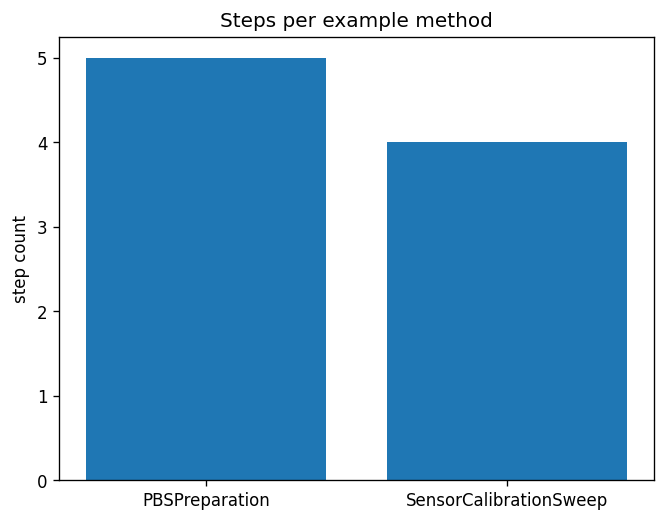
\includegraphics[keepaspectratio,alt={Steps per example method: a bar chart built from len(plan.steps) for each plan in output/data/compiled\_plans.json, plotted by scripts/methods\_analysis.py.}]{../figures/step_counts.png}}
\caption{Steps per example method: a bar chart built from
\protect\texttt{len(plan.steps)} for each plan in
\protect\breaktt{output/data/compiled\_plans.json}, plotted by
\protect\breaktt{scripts/methods\_analysis.py}.}\label{fig:step_counts}
\end{figure}

\subsection{Validation gates}\label{validation-gates}

Across both methods, the analysis script tallies 8 of 8 staged-gate
evaluations passing (\texttt{run\_all\_gates} \texorpdfstring{\ensuremath{\times}}{x} 2 methods \texorpdfstring{\ensuremath{\times}}{x} 4 gates
each). Every gate result is written to
\breaktt{output/reports/gate\_report.json} --- neither method in this
manuscript is hand-picked to pass; both worked examples are constructed
to satisfy the structural, semantic, plan, and target gates by design,
since \texttt{compile\_method} raises \breaktt{MethodValidationError} and
halts the pipeline on any gate failure.

\subsection{Determinism}\label{determinism}

Recompiling each example method twice and comparing \texttt{plan\_hash}
values yields: \textbf{determinism check = Yes}. This is a live
re-compilation comparison performed by
\breaktt{src/manuscript\_variables.py} at manuscript-build time, not a
value asserted once and then transcribed --- the same property
sec.~\ref{sec:methodology} claims for \texttt{compile\_method} is
checked again here, independently, against the live build.

\subsection{Provenance demonstration}\label{provenance-demonstration}

\breaktt{scripts/methods\_analysis.py} appends a 3-record demonstration
hash-chain for one value (\breaktt{calibration\_offset}) through
\texttt{DECLARED} \texorpdfstring{\ensuremath{\to}}{->} \texttt{CALIBRATED} \texorpdfstring{\ensuremath{\to}}{->} \texttt{VERIFIED} tiers and
writes the result of \texttt{verify\_chain} to
\breaktt{output/reports/trust\_chain\_report.json}: \textbf{chain
verified = Yes}.

\subsection{Validation}\label{validation}

The results were validated through the zero-mock \texttt{tests/} suite:

\begin{itemize}
\tightlist
\item
  \textbf{Library tests} assert exact gate outcomes, scheduling order,
  and plan-hash determinism against real \texttt{Method} fixtures,
  including one fixture per gate-failure mode.
\item
  \textbf{Script test} runs \breaktt{run\_methods\_analysis()} against a
  temporary output root and confirms real worklist/CSV/Mermaid/JSON
  artifacts, reports, and a real PNG figure are written.
\item
  \textbf{Manuscript-variable test} confirms every generated-variable
  name used in \texttt{manuscript/*.md} is emitted by
  \breaktt{generate\_variables}.
\end{itemize}

All tests pass with coverage exceeding the 90\% project gate, with no
mocks.

\subsection{Discussion}\label{discussion}

The results confirm the pipeline end to end: both worked examples pass
every staged gate, compile deterministically, and produce a stable plan
hash across repeated builds. The same \breaktt{src/methods\_dsl/}
functions back the analysis script, the test suite, and this manuscript
--- which is the architectural point of the exemplar. Because every
number here is produced by a tested function and regenerated on demand,
the prose describes structure and provenance rather than transcribing
values that would drift the moment the example methods changed.

\newpage

\section{Conclusion}\label{sec:conclusion}

This paper presented a small, tested domain language for specifying
controlled methods, informed by BPL's \citep{bpl2026} domain-language
design for laboratory protocols and generalized to any controlled
procedure. It validates a simple proposition: a controlled vocabulary
expressed as typed, validated dataclasses --- not a parsed text grammar
--- is sufficient to reproduce BPL's core safety properties at a scope
appropriate for a template exemplar.

\subsection{Exemplar achievements}\label{exemplar-achievements}

Operating as the methods-paper exemplar for the Research Project
Template methodology, the project deployed the three foundational
pillars:

\begin{enumerate}
\def\labelenumi{\arabic{enumi}.}
\tightlist
\item
  \textbf{\breaktt{src/methods\_dsl/} library}: a controlled vocabulary,
  a dimensional unit system, four staged validation gates, a
  deterministic compiler, and four export formats --- with no plotting,
  no file I/O, and (with one declared logging exception) no
  \texttt{infrastructure} imports.
\item
  \textbf{\texttt{tests/} integrity}: a zero-mock suite over real
  \texttt{Method} fixtures covering the success path and every
  gate-failure mode, under a \texorpdfstring{\textgreater{}=}{>=}90\% project coverage gate.
\item
  \textbf{\texttt{docs/} knowledge operations}: the correspondence with
  BPL's pipeline, testing philosophy, and operational rules that keep
  the library, scripts, and manuscript aligned.
\end{enumerate}

\subsection{Technical contributions}\label{technical-contributions}

\subsubsection{Controlled vocabulary in code, not a
parser}\label{controlled-vocabulary-in-code-not-a-parser}

The hallmark of this exemplar is the design choice it demonstrates: a
\texttt{.bpl} file's text grammar buys generality this template does not
need, while a frozen-dataclass model buys construction-time validation
(\texttt{\_\_post\_init\_\_}) that a parsed AST would have to re-derive.
The controlled vocabulary's discipline lives in the \emph{types}, not in
concrete syntax.

\subsubsection{Honest handling of trust
boundaries}\label{honest-handling-of-trust-boundaries}

\texttt{trust.py}'s hash-chain documents its own limit explicitly: it
detects in-chain tampering but cannot detect a chain rewritten from
record zero. This makes the provenance guarantee a visible, testable
property rather than an implied cryptographic guarantee the
implementation does not actually provide.

\subsection{Key insights}\label{key-insights}

\begin{enumerate}
\def\labelenumi{\arabic{enumi}.}
\tightlist
\item
  \textbf{Determinism follows from explicit tie-breaking}: Kahn's
  algorithm \citep{kahn1962topological} alone does not guarantee a
  stable schedule across runs --- the ascending-\texttt{step\_id}
  tie-break is what makes \texttt{plan\_hash} reproducible, and
  sec.~\ref{sec:results} checks this live rather than asserting it.
\item
  \textbf{Staged short-circuit avoids misleading errors}: running
  \texttt{plan\_gate} and \texttt{target\_gate} against a structurally
  invalid method would report noise, not signal ---
  \texttt{run\_all\_gates} short-circuits after the first two gates for
  exactly this reason.
\item
  \textbf{A controlled vocabulary generalizes by restraint, not by
  expansion}: \breaktt{SensorCalibrationSweep} reuses every
  \texttt{StepKind} and \texttt{Target} the wet-lab-flavored
  \texttt{PBSPreparation} example uses; nothing was added to support a
  second domain.
\end{enumerate}

\subsection{Future extensions}\label{future-extensions}

This foundation could be extended to:

\begin{itemize}
\tightlist
\item
  \textbf{A real \texttt{.bpl}-style parser}: add
  \texttt{grammar/}/\texttt{parser/}/\texttt{transformer/} stages ahead
  of the existing \texttt{model.py}, reusing every downstream gate and
  the compiler unchanged.
\item
  \textbf{More backends}: a \texttt{robot} execution target with
  capability-aware lowering, mirroring BPL's Biomek translation layer.
\item
  \textbf{A capability registry}: per-target primitive support
  declarations, generalizing BPL's \texttt{capabilities/} registry and
  \breaktt{bplc\ capabilities} report.
\end{itemize}

\subsection{Final assessment}\label{final-assessment}

The \breaktt{template\_methods\_paper} tree is the canonical reference
for how a methods paper --- a manuscript whose subject is a methodology
--- stays synchronized with the code implementing that methodology
across rebuilds. The pipeline compiled both worked example methods,
wrote \breaktt{output/data/compiled\_plans.json},
\breaktt{output/reports/gate\_report.json}, and
\breaktt{output/reports/trust\_chain\_report.json}, and rendered this
markdown together with \texttt{config.yaml} into PDF.

\newpage

\section{Experimental Setup}\label{sec:experimental_setup}

This section details the controlled vocabulary, worked examples, and
software environment used to produce the results.

\subsection{Controlled vocabulary}\label{controlled-vocabulary}

The DSL's vocabulary is declared once in code and consulted by every
gate and the compiler --- never re-declared per method:

{\def\LTcaptype{none} % do not increment counter
\begin{longtable}[]{@{}
  >{\raggedright\arraybackslash}p{(\linewidth - 4\tabcolsep) * \real{0.3333}}
  >{\raggedright\arraybackslash}p{(\linewidth - 4\tabcolsep) * \real{0.3333}}
  >{\raggedright\arraybackslash}p{(\linewidth - 4\tabcolsep) * \real{0.3333}}@{}}
\toprule\noalign{}
\begin{minipage}[b]{\linewidth}\raggedright
Module
\end{minipage} & \begin{minipage}[b]{\linewidth}\raggedright
Declares
\end{minipage} & \begin{minipage}[b]{\linewidth}\raggedright
Cardinality
\end{minipage} \\
\midrule\noalign{}
\endhead
\bottomrule\noalign{}
\endlastfoot
\breaktt{src/methods\_dsl/vocabulary.py} & \texttt{StepKind},
\texttt{Target}, \texttt{target\_accepts} & 9 step kinds, 3 targets \\
\breaktt{src/methods\_dsl/units.py} & \texttt{Dimension},
\texttt{Quantity}, the unit table & 18 controlled units across 7
dimensions \\
\breaktt{src/methods\_dsl/validation.py} & The four staged gates & 4
gates, fixed order \\
\end{longtable}
}

\subsection{Worked examples}\label{worked-examples}

\breaktt{all\_example\_methods()}
(\breaktt{src/methods\_dsl/examples\_methods.py}) returns 2 methods:

{\def\LTcaptype{none} % do not increment counter
\begin{longtable}[]{@{}
  >{\raggedright\arraybackslash}p{(\linewidth - 6\tabcolsep) * \real{0.2500}}
  >{\raggedright\arraybackslash}p{(\linewidth - 6\tabcolsep) * \real{0.2500}}
  >{\raggedright\arraybackslash}p{(\linewidth - 6\tabcolsep) * \real{0.2500}}
  >{\raggedright\arraybackslash}p{(\linewidth - 6\tabcolsep) * \real{0.2500}}@{}}
\toprule\noalign{}
\begin{minipage}[b]{\linewidth}\raggedright
Method
\end{minipage} & \begin{minipage}[b]{\linewidth}\raggedright
Domain
\end{minipage} & \begin{minipage}[b]{\linewidth}\raggedright
Target
\end{minipage} & \begin{minipage}[b]{\linewidth}\raggedright
Notable structure
\end{minipage} \\
\midrule\noalign{}
\endhead
\bottomrule\noalign{}
\endlastfoot
\texttt{PBSPreparation} & Wet-lab bench preparation (BPL's own domain;
an original example) & \texttt{HUMAN} & A strict 5-step linear chain
with a final \texttt{VALIDATE} step \\
\breaktt{SensorCalibrationSweep} & Instrument calibration (a non-biology
controlled procedure) & \texttt{AUTOMATED} & Mixed automated
\texttt{MEASURE}/\texttt{COMPUTE} steps and a \texttt{HUMAN}
\texttt{ANNOTATE} sign-off step \\
\end{longtable}
}

The second example exists specifically to demonstrate that the
controlled vocabulary generalizes beyond wet-lab protocols, as
sec.~\ref{sec:introduction} claims.

\subsection{Pipeline conditions}\label{pipeline-conditions}

The experiment overlay (\breaktt{experiment\_plan.yaml}) declares three
conditions:

\begin{itemize}
\tightlist
\item
  \textbf{declared\_method} (reference) --- a method constructed
  directly as Python objects, before any validation gate has run.
\item
  \textbf{validated\_method} (proposed) --- the same method after
  passing all four staged gates and deterministic compilation to a
  scheduled \texttt{Plan}.
\item
  \textbf{automated\_target\_variant} (variant) ---
  \texttt{PBSPreparation}'s steps recompiled against an
  \texttt{AUTOMATED} execution target, ablating the target-compatibility
  gate's \texttt{HUMAN}/\texttt{AUTOMATED} step boundary (a
  \texttt{HUMAN} method's steps must all be \texttt{HUMAN}-compatible;
  an \texttt{AUTOMATED} method's steps may be either).
\end{itemize}

The primary metric is gate pass rate: the fraction of staged-gate
evaluations a method's steps satisfy.

\subsection{Computational environment}\label{computational-environment}

\begin{itemize}
\tightlist
\item
  \textbf{Language}: Python 3.12.13 on Darwin arm64 (see root
  \texttt{pyproject.toml} for the supported version range).
\item
  \textbf{Core dependencies}: \texttt{pyyaml}, \texttt{matplotlib}
  (declared in \breaktt{domain\_profile.yaml::required\_packages}); the
  DSL library itself (\breaktt{src/methods\_dsl/}) has zero third-party
  dependencies beyond the standard library, with one declared
  \texttt{infrastructure} logging exception (\texttt{\_logging.py}).
\item
  \textbf{Headless plotting}: the analysis script sets
  \texttt{MPLBACKEND=Agg} before importing matplotlib.
\end{itemize}

\subsection{Pipeline ordering}\label{pipeline-ordering}

The typical analysis order is:

\begin{enumerate}
\def\labelenumi{\arabic{enumi}.}
\tightlist
\item
  \breaktt{scripts/methods\_analysis.py} --- compiles every example
  method, runs all gates, exports worklist/CSV/Mermaid/JSON per method,
  demonstrates the provenance hash-chain, and writes
  \breaktt{../figures/step\_counts.png}, printing each output path for
  manifest collection.
\item
  \breaktt{scripts/z\_generate\_manuscript\_variables.py} --- reads
  \breaktt{manuscript/config.yaml} and the analysis outputs, then
  resolves every generated variable in \texttt{manuscript/*.md}.
\item
  PDF rendering reads the resolved manuscript tree so figure paths and
  prose match the analysis that just completed.
\end{enumerate}

\subsection{Relation to results}\label{relation-to-results}

{\def\LTcaptype{none} % do not increment counter
\begin{longtable}[]{@{}
  >{\raggedright\arraybackslash}p{(\linewidth - 4\tabcolsep) * \real{0.3333}}
  >{\raggedright\arraybackslash}p{(\linewidth - 4\tabcolsep) * \real{0.3333}}
  >{\raggedright\arraybackslash}p{(\linewidth - 4\tabcolsep) * \real{0.3333}}@{}}
\toprule\noalign{}
\begin{minipage}[b]{\linewidth}\raggedright
Result (sec.~\ref{sec:results})
\end{minipage} & \begin{minipage}[b]{\linewidth}\raggedright
Producing function (\breaktt{src/methods\_dsl/})
\end{minipage} & \begin{minipage}[b]{\linewidth}\raggedright
Primary inputs
\end{minipage} \\
\midrule\noalign{}
\endhead
\bottomrule\noalign{}
\endlastfoot
Compiled-plan summary & \breaktt{compile\_method()} &
\breaktt{all\_example\_methods()} \\
Step-count figure & \texttt{len(plan.steps)} per method &
\breaktt{output/data/compiled\_plans.json} \\
Gate pass tally & \texttt{run\_all\_gates()} & Each example method \\
Determinism check & \breaktt{compile\_method()} called twice &
\breaktt{all\_example\_methods()} \\
Trust-chain verification & \texttt{append\_record()} /
\texttt{verify\_chain()} & Demonstration chain in
\breaktt{scripts/methods\_analysis.py} \\
\end{longtable}
}

This table is descriptive documentation only; it is not executed as code
during the build.

\newpage

\section{Reproducibility}\label{sec:reproducibility}

This section explains how to regenerate every artifact in the study from
a clean checkout. The exemplar's reproducibility guarantee is
structural: each result is produced by a tested function and a thin
script, then injected into the manuscript by generated-variable
substitution --- never transcribed by hand.

\subsection{How to regenerate
everything}\label{how-to-regenerate-everything}

From the repository root:

\begin{Shaded}
\begin{Highlighting}[]
\CommentTok{\# 1. Run the analysis (compiles methods, exports artifacts, writes figure + reports)}
\ExtensionTok{uv}\NormalTok{ run python projects/templates/template\_methods\_paper/scripts/methods\_analysis.py}

\CommentTok{\# 2. Run the test suite with the coverage gate}
\ExtensionTok{uv}\NormalTok{ run pytest projects/templates/template\_methods\_paper/tests }\DataTypeTok{\textbackslash{}}
    \AttributeTok{{-}{-}cov}\OperatorTok{=}\NormalTok{projects/templates/template\_methods\_paper/src }\AttributeTok{{-}{-}cov{-}fail{-}under}\OperatorTok{=}\NormalTok{90}

\CommentTok{\# 3. Generate and inject manuscript variables}
\ExtensionTok{uv}\NormalTok{ run python projects/templates/template\_methods\_paper/scripts/z\_generate\_manuscript\_variables.py}

\CommentTok{\# 4. Render the manuscript}
\ExtensionTok{uv}\NormalTok{ run python scripts/03\_render\_pdf.py }\AttributeTok{{-}{-}project}\NormalTok{ templates/template\_methods\_paper}
\end{Highlighting}
\end{Shaded}

Or, end to end via the orchestrated pipeline:

\begin{Shaded}
\begin{Highlighting}[]
\ExtensionTok{uv}\NormalTok{ run python scripts/execute\_pipeline.py }\AttributeTok{{-}{-}project}\NormalTok{ templates/template\_methods\_paper }\AttributeTok{{-}{-}core{-}only}
\end{Highlighting}
\end{Shaded}

\subsection{Generated artifact
registry}\label{generated-artifact-registry}

The analysis script writes the following artifacts under
\breaktt{projects/templates/template\_methods\_paper/output/}:

{\def\LTcaptype{none} % do not increment counter
\begin{longtable}[]{@{}
  >{\raggedright\arraybackslash}p{(\linewidth - 2\tabcolsep) * \real{0.5000}}
  >{\raggedright\arraybackslash}p{(\linewidth - 2\tabcolsep) * \real{0.5000}}@{}}
\toprule\noalign{}
\begin{minipage}[b]{\linewidth}\raggedright
Artifact
\end{minipage} & \begin{minipage}[b]{\linewidth}\raggedright
Produced by
\end{minipage} \\
\midrule\noalign{}
\endhead
\bottomrule\noalign{}
\endlastfoot
\breaktt{data/pbspreparation\_worklist.md},
\breaktt{data/pbspreparation\_plan.csv},
\breaktt{data/pbspreparation\_graph.mmd},
\breaktt{data/pbspreparation\_plan.json} & \breaktt{compile\_method()} +
exporters, for \texttt{PBSPreparation} \\
\breaktt{data/sensorcalibrationsweep\_worklist.md},
\breaktt{data/sensorcalibrationsweep\_plan.csv},
\breaktt{data/sensorcalibrationsweep\_graph.mmd},
\breaktt{data/sensorcalibrationsweep\_plan.json} &
\breaktt{compile\_method()} + exporters, for
\breaktt{SensorCalibrationSweep} \\
\breaktt{data/compiled\_plans.json} & Per-method plan summary, consumed
by \breaktt{src/manuscript\_variables.py} \\
\breaktt{reports/gate\_report.json} & \texttt{run\_all\_gates()} tally
across both methods \\
\breaktt{reports/trust\_chain\_report.json} &
\texttt{append\_record()}/\texttt{verify\_chain()} demonstration
chain \\
\breaktt{figures/step\_counts.png} & Step-count bar chart \\
\breaktt{data/manuscript\_variables.json} & Every generated-variable
value, written by \breaktt{z\_generate\_manuscript\_variables.py} \\
\end{longtable}
}

The \texttt{output/} tree is disposable and regenerated on every run; it
is not the source of truth.

\subsection{Determinism}\label{determinism-1}

\begin{itemize}
\tightlist
\item
  \breaktt{compile\_method()} is deterministic by construction: the plan
  hash is computed from a canonical, sort-keys JSON payload over
  \texttt{method\_name}, \texttt{method\_version}, \texttt{target}, and
  each scheduled step's identifying fields --- never from a wall-clock
  timestamp or a UUID.
\item
  \breaktt{topological\_order()} breaks scheduling ties by ascending
  \texttt{step\_id}, so the same \texttt{Method} object always yields
  the same step order across processes and platforms.
\item
  Yes --- \breaktt{src/manuscript\_variables.py::generate\_variables}
  recompiles every example method twice at manuscript-build time and
  compares hashes live, so this guarantee is checked on every build, not
  merely asserted once in a test.
\end{itemize}

\subsection{Verification (no hand-transcribed
numbers)}\label{verification-no-hand-transcribed-numbers}

Every quantitative claim in sec.~\ref{sec:results} is either a generated
variable sourced from a live analysis output or registered in
\breaktt{data/claim\_ledger.yaml} for evidence-registry validation. The
manuscript intentionally does not hand-transcribe volatile values, so
prose and artifacts cannot disagree. Configuration provenance is itself
injected: \breaktt{2107a29383e5e491} is the SHA-256 of
\breaktt{manuscript/config.yaml} at build time, and
\breaktt{2026-06-30T21:41:36Z} records when the variables were generated
(honoring \breaktt{SOURCE\_DATE\_EPOCH} for byte-reproducible builds).

\newpage

\section{Scope, Related Work, and Positioning}\label{sec:scope}

This section situates the exemplar and states explicit boundaries. The
goal is not to compete with BPL's full compiler pipeline \citep{bpl2026}
--- a about 32,000-line implementation with a Lark grammar, a
robot backend, and a hash-chained audit/compliance layer --- but to show
how a minimal, test-backed subset of BPL's domain-language design fits
the template's reproducibility and rendering stack
\citep{peng2011reproducible}, generalized from wet-lab protocols to any
controlled procedure.

\subsection{Domain-specific languages for controlled
procedures}\label{domain-specific-languages-for-controlled-procedures}

Encoding a procedure as a program rather than free text is a
long-standing software-engineering pattern: Fowler's treatment of
domain-specific languages \citep{fowler2010dsl} frames the general case
--- a notation restricted to exactly the concepts a domain needs. BPL
\citep{bpl2026} applies this specifically to laboratory protocols,
adding biology-native types (reagents, labware, MW-aware
concentrations), staged validation, and deterministic compilation to a
robot or human execution target. The present manuscript restricts
attention to the parts of that design that generalize beyond biology: a
controlled vocabulary of step intents, a small dimensional-safety unit
system, staged validation gates, and deterministic compilation to a
hashed plan.

\subsection{What this exemplar does not implement (out of
scope)}\label{what-this-exemplar-does-not-implement-out-of-scope}

\begin{enumerate}
\def\labelenumi{\arabic{enumi}.}
\tightlist
\item
  \textbf{A text grammar and parser.} BPL parses \texttt{.bpl} source
  through a Lark grammar into a typed AST. This exemplar constructs a
  \texttt{Method} directly as frozen Python dataclasses --- no concrete
  syntax, no parser, no AST layer.
\item
  \textbf{Biology-native types.} BPL's unit system includes MW-aware
  concentration conversions and reagent physical-form metadata
  (\texttt{cas}, \texttt{physical\_form}). This exemplar's
  \texttt{units.py} implements only the dimensional-safety subset (mass,
  volume, temperature, time, concentration, count, dimensionless) needed
  to demonstrate the ``the type system catches \texttt{mL\ +\ g}''
  guarantee.
\item
  \textbf{A robot backend.} BPL lowers intents to Biomek i7 primitives
  (\texttt{aspirate}, \texttt{dispense}, \texttt{pick\_tips}). This
  exemplar's \breaktt{Target.AUTOMATED} has no backend-specific lowering
  stage; it is a scheduling and gate-compatibility concept only.
\item
  \textbf{Cryptographic audit guarantees.} \texttt{trust.py}'s
  hash-chain is deliberately scoped to the same honest boundary BPL
  itself claims: a consistency check against accidental corruption, not
  a tamper-proof guarantee against an actor with write access to the
  entire chain.
\item
  \textbf{SOP-to-DSL generation.} BPL includes an agentic workflow that
  translates natural-language SOPs into validated \texttt{.bpl}
  programs. This exemplar's worked examples are hand-authored Python,
  not generated.
\end{enumerate}

\subsection{What this project proves about the
template}\label{what-this-project-proves-about-the-template}

The validation and compilation steps here are a deliberately small
subset of BPL's. The \textbf{non-standard} contribution is procedural:
the same tested functions in \breaktt{src/methods\_dsl/} back the
analysis script, the test suite, and this manuscript, so the
compiled-plan table and the figure always refer to the same code. That
pattern --- and the specific generalization from a biology-only domain
language to a domain-neutral one --- is what downstream projects should
copy, whether the controlled procedure is a wet-lab protocol, an
instrument calibration sweep, or a computational pipeline.

\subsection{Explicit limitations}\label{explicit-limitations}

\begin{enumerate}
\def\labelenumi{\arabic{enumi}.}
\tightlist
\item
  \textbf{Two worked examples}: \texttt{PBSPreparation} and
  \breaktt{SensorCalibrationSweep} exercise every gate-success path but
  are not a corpus; gate-failure coverage instead lives in
  \breaktt{tests/conftest.py}'s dedicated fixtures.
\item
  \textbf{No backend lowering}: \texttt{Target} selects a compatibility
  class, not a concrete execution backend; no robot or simulation
  runtime exists in this exemplar.
\item
  \textbf{Unit table, not a full unit library}: seven dimensions and a
  fixed unit table, not a general-purpose dimensional-analysis library
  like \texttt{pint}.
\item
  \textbf{No persistence layer}: \texttt{trust.py}'s hash-chain lives in
  memory for the duration of one script run; this exemplar does not
  implement durable storage for a real audit trail.
\end{enumerate}

These limitations are intentional: they narrow the surface so that the
reproducibility concerns --- tested functions, a thin script, and
generated-variable-injected prose --- remain visible rather than buried
under a compiler implementation at BPL's full scale.

\newpage

\section{References}\label{sec:references}

Bibliography lives in
\href{references.bib}{\breaktt{manuscript/references.bib}} and is read by
Pandoc during PDF render. The build pipeline invokes Pandoc with
\texttt{-\/-natbib}, so every \texttt{{[}@key{]}} citation in the
manuscript is rewritten to the appropriate
\texttt{\textbackslash{}cite\{\}}/\texttt{\textbackslash{}citep\{\}}/\texttt{\textbackslash{}citet\{\}}
LaTeX command and resolved against the bib file.

To validate that \texttt{references.bib} is syntactically clean and
contains the required fields per entry type:

\begin{Shaded}
\begin{Highlighting}[]
\ExtensionTok{uv}\NormalTok{ run python }\AttributeTok{{-}m}\NormalTok{ infrastructure.reference.citation.cli validate }\DataTypeTok{\textbackslash{}}
\NormalTok{    projects/templates/template\_methods\_paper/manuscript/references.bib }\AttributeTok{{-}{-}strict}
\end{Highlighting}
\end{Shaded}




\clearpage

\bibliography{references}
\end{document}
